\section{Use Cases}\label{Use Cases}

In this chapter, the typical usages of the N2Sky platform will be described.

\subsection{N2Sky as a Learning Platform}\label{N2Sky as a learning platform}

The N2Sky platform was developed originally in university for students starting from N2Grid \cite{schikuta2004n2grid}. Today, N2Sky is still mainly working for students and people, who are interested in neural network field without deep knowledge of it. 

The most students and young people are using mobile smart devices like mobile phones or tablets for multiple purposes. The N2Sky platform is fully supporting any kind of device, that is why by assumption the students will use the mobile device in this use case. 

In figure \ref{fig:use_case_student} the typical student use case is displayed.


\begin{figure}[htbp]
\begin{center}
  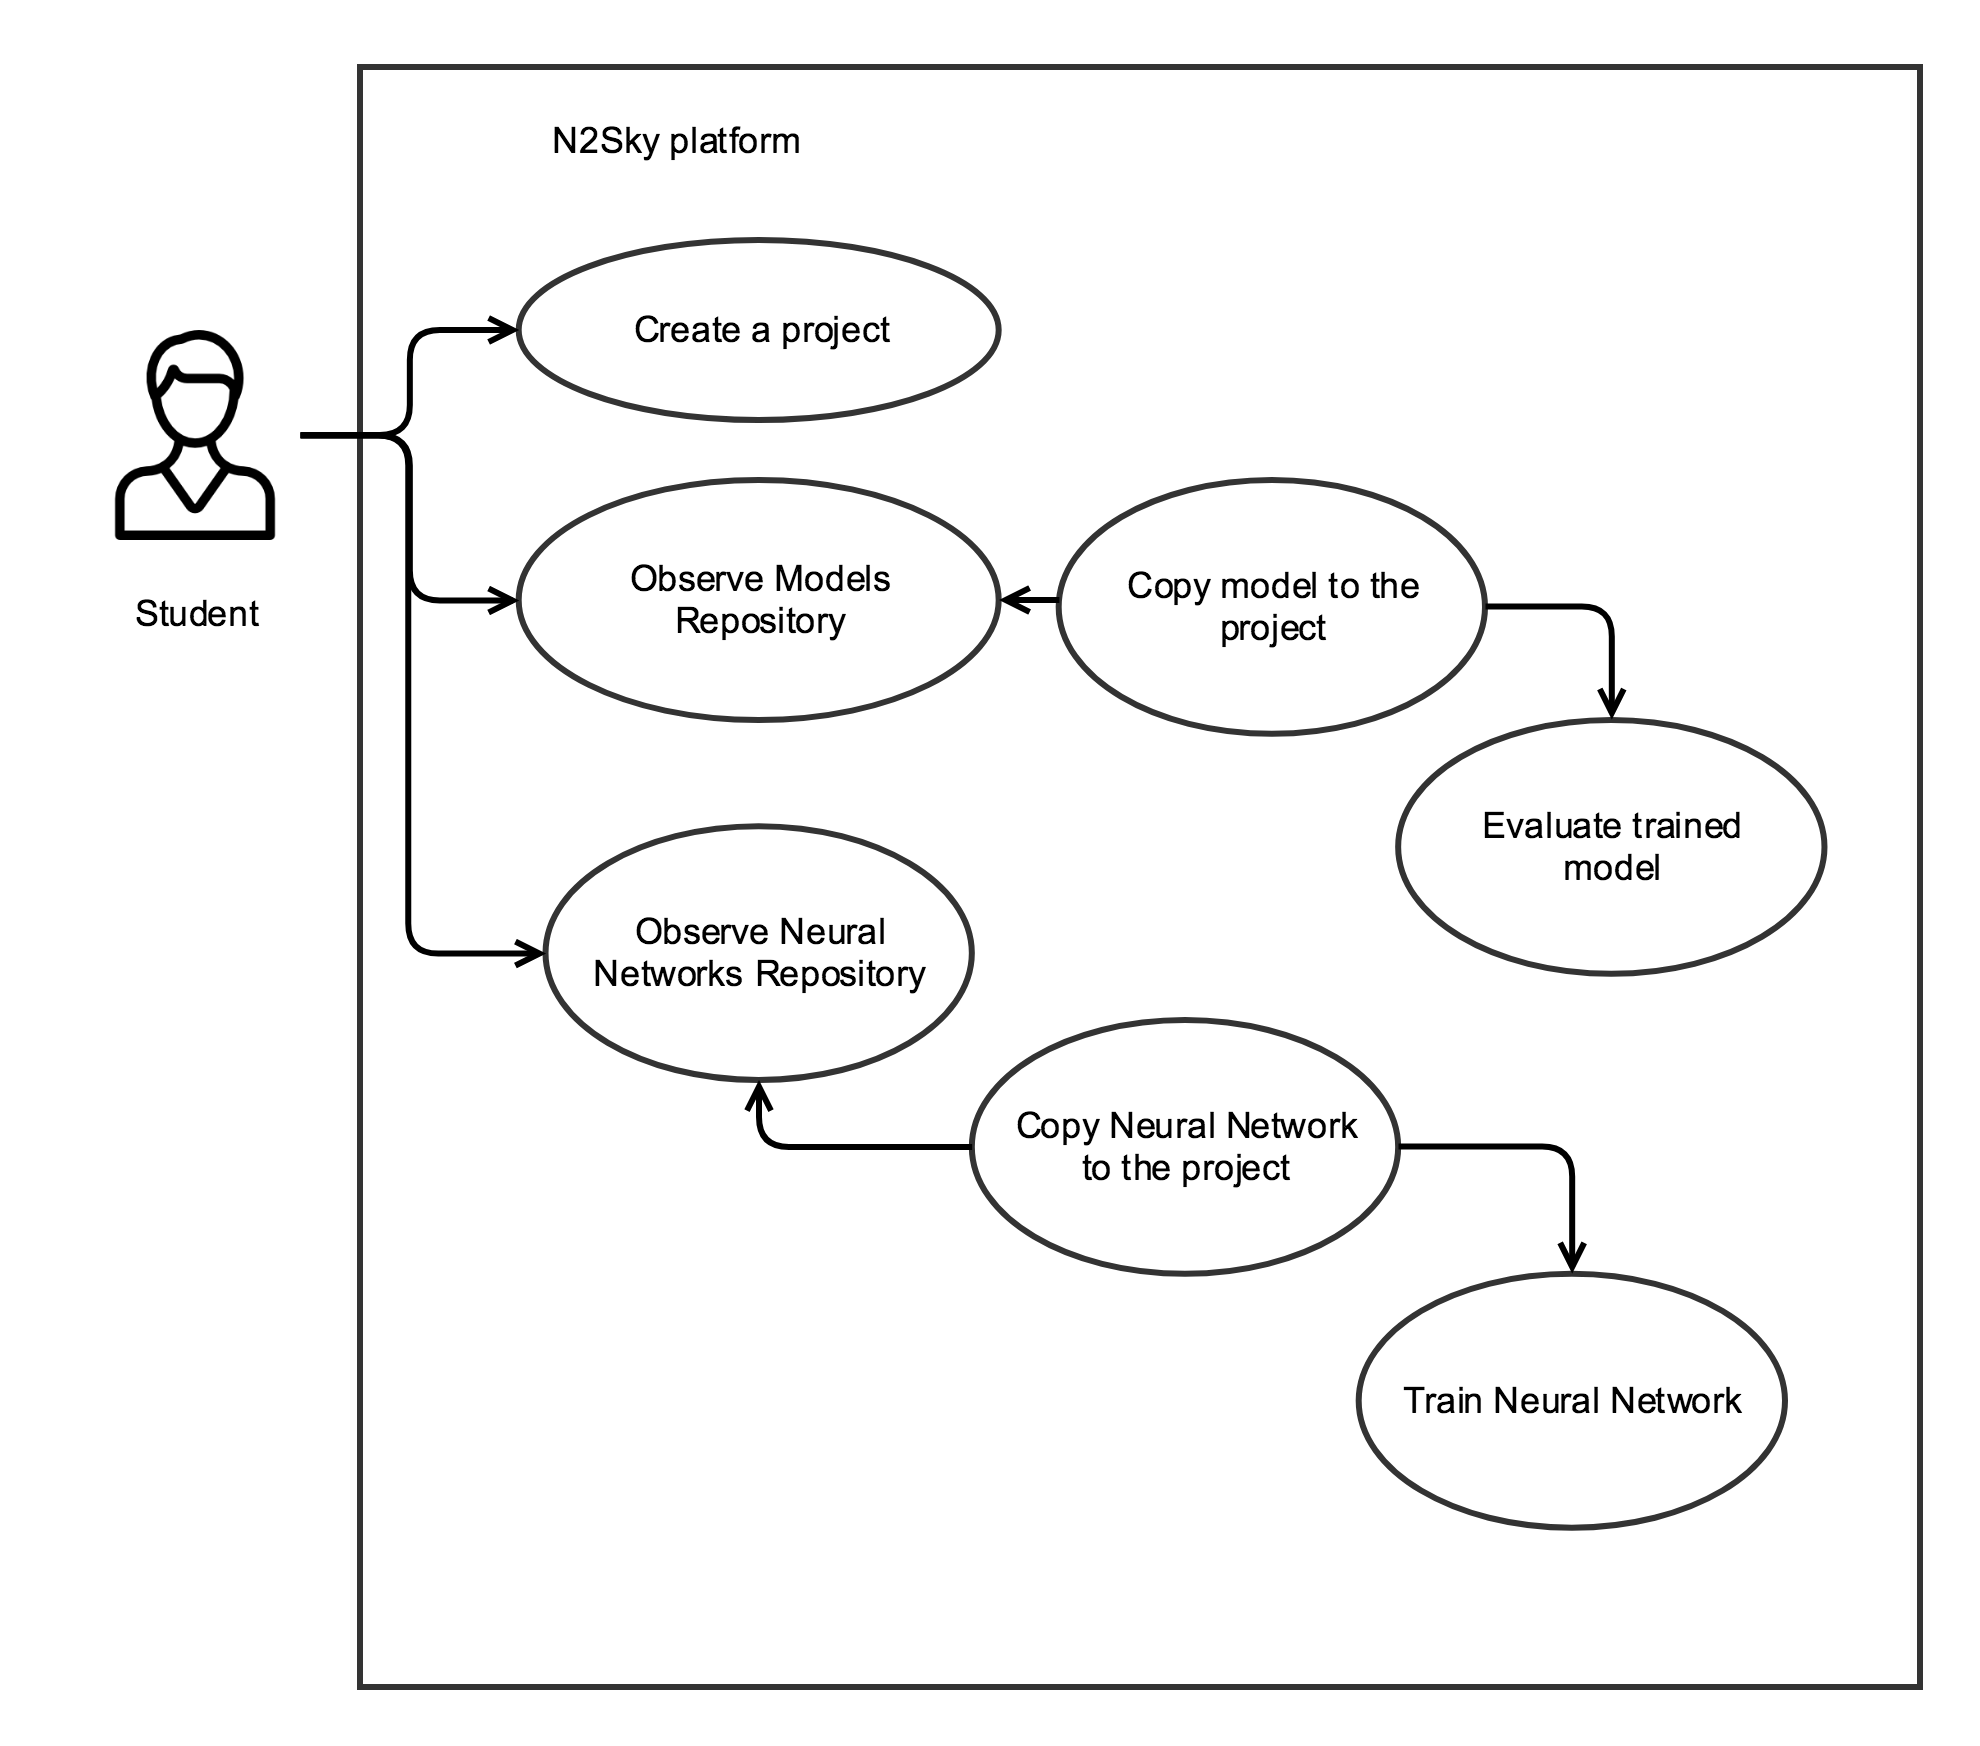
\includegraphics[width=\linewidth]{components/usecase/img/use_case_student.png}
  \caption{Use Case of typical arbitrary user behaviour}
  \label{fig:use_case_student}
\end{center}
\end{figure} 

The student is an arbitrary user. The detailed information of main functions of the users are described in \autoref{User Roles}. 

This user can create a project, which it will be in the focus after the first login. The project is a collection of the created or copied neural networks and trained models. After creating the project, the arbitrary user does not have to develop anything or know any programming language in order to use the N2Sky platform. The student can search for an existing neural network in the Neural Networks repository or for existing trained model in the Models Repository. 

The user can reuse, namely copy existing neural network or trained model. Before doing this, the arbitrary user can check the details of the neural network or trained model.  
The user can observe how the neural network was behaving and study already existing trained models. 

After copying the neural network or the trained model, the arbitrary user can use the default data across the whole training and evaluation process. The main idea is that the user will learn. The user can test different parameters and observe the results. With this approach, the student can study the behaviour of the neural network.

All these procedures, can be performed directly from the mobile device.  Every action is intuitive and fully adapted to the device type.

\subsection{Developing the Neural Network with N2Sky}\label{Developing the neural network with N2Sky}

The typical use case when the user has experience in neural network field or the user already developed his own neural network and wants to test it, is displayed in figure \ref{fig:user_case_engin}.

\begin{figure}[htbp]
\begin{center}
  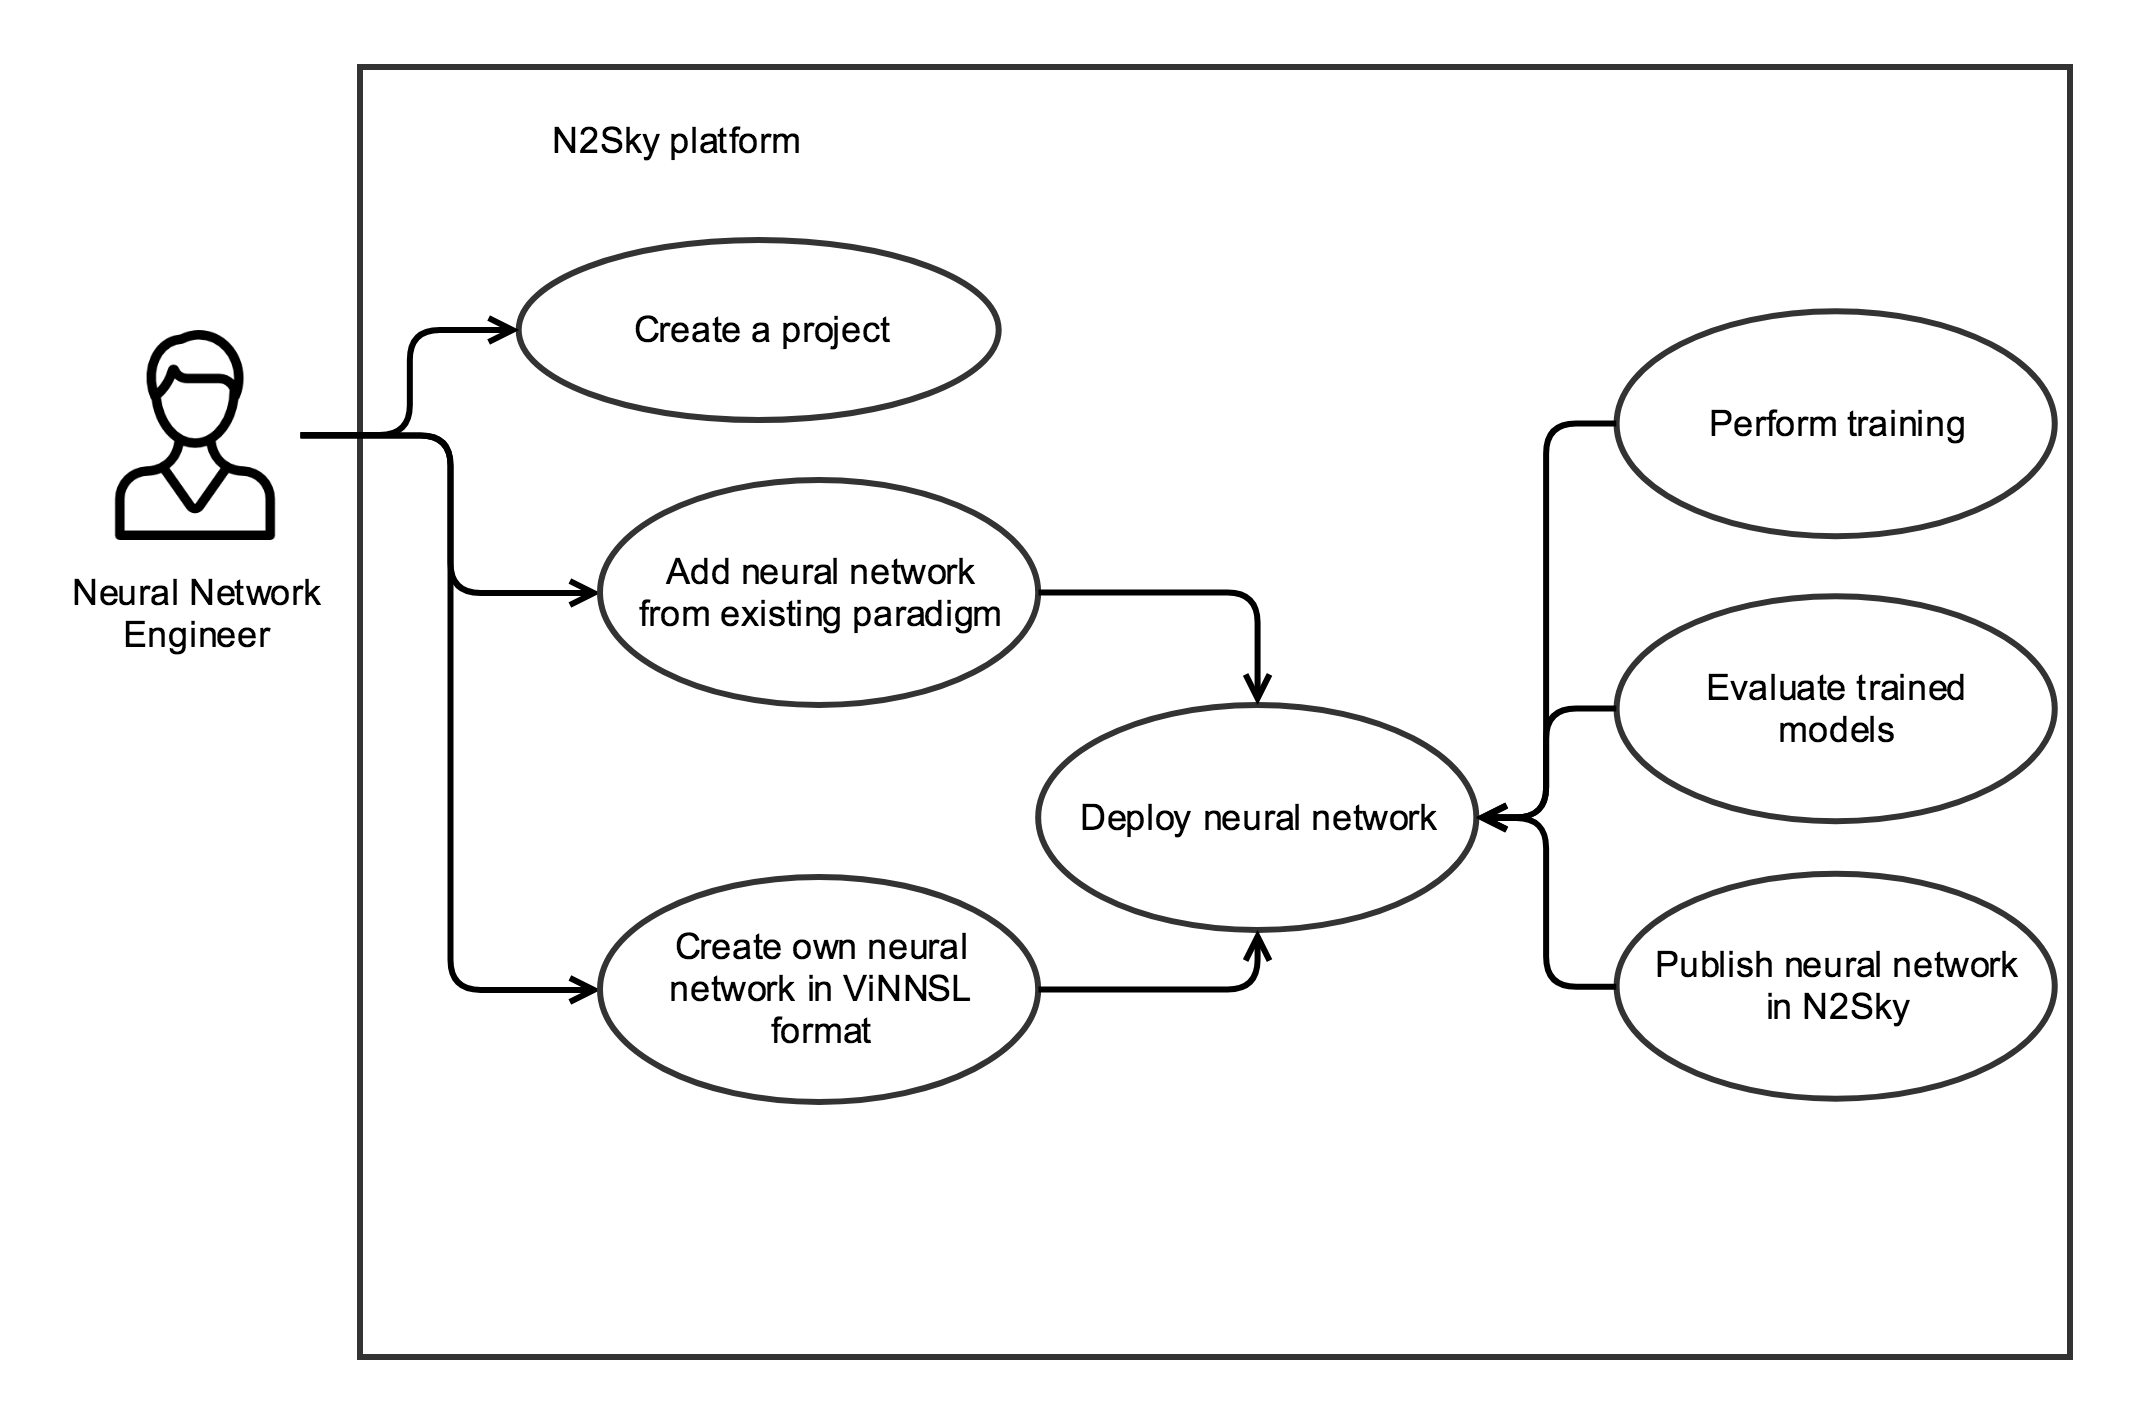
\includegraphics[width=\linewidth]{components/usecase/img/user_case_engin.png}
  \caption{Use Case. Developing the neural network with N2Sky.}
  \label{fig:user_case_engin}
\end{center}
\end{figure} 

This user operates differently with N2Sky. In most cases, he will use the desktop version of the application. 
This category of users can be more professional. Some users could use technical jargon while others know just the neural network field more theoretically, then practically. More details about user roles are described in \autoref{User Roles}. 

If the user knows the field theoretically and does not have experience in the actual creation of the neural network, N2Sky gives such a possibility. With the neural network generator, the user can choose existing paradigms and create the neural network with a few simple steps. 

If the user has experience in the actual creation of the neural network, he can write a ViNNSL formatted neural network description and upload it to the N2Sky platform. Since the user has developed neural networks before, he could also use his own cloud in order to deploy it. 

The next steps are the same in case if the user creates the neural network from the paradigm or upload his own neural network on the N2Sky platform:

\begin{itemize}
\item \emph{Perform training.}  Unlike arbitrary users, the neural network engineers or the contributor users can use own training data. 
\item \emph{Evaluate the trained models.} The users can perform tests against trained model with their own testing data.
\item \emph{Publish neural network on N2Sky} in order to make it available in the neural network repository. When the neural network will be published, arbitrary users can reuse it for their own need. 
\end{itemize}


